\documentclass[a4paper,12pt]{article}   % papír A4, písmo 12 bodu
\usepackage[utf8x]{inputenc}            %kodovaní UTF-8
\usepackage{ucs}                        %kodovani unicode
\usepackage[czech]{babel}               %podpora cestiny
\usepackage[T1]{fontenc}                %pouzij variantu pisma T1 (hacky, carky)
\usepackage[left=2.5cm,right=1.5cm,top=2.5cm,bottom=2.5cm]{geometry} %okraje stranky
\usepackage{amsmath,amsfonts,amssymb}   %podpora matematiky
\usepackage{gensymb,marvosym}           %symboly celsius (\celsius) apod.
%\usepackage{mathptmx}                   %font Times New Roman s~podporou matematiky
\usepackage{times}                      %font Times New Roman (matematika pismem Computer Modern) 
\usepackage{parskip}                    %mezera mezi odstavci
%\usepackage[document]{ragged2e}         %text zarovany vlevo
\usepackage[none]{hyphenat} \sloppy     %slova nedelit a~nepretekat
\usepackage{titlesec}
\setcounter{secnumdepth}{4}
\clubpenalty 10000                      %kontrolovat sirotky
\widowpenalty 10000                     %kontrolovat vdovy
\usepackage{setspace} \onehalfspacing   %podpora pro zmenu radkovani + radkovani 1,5
\usepackage{enumerate}                  %podpora pro zmenu cislovani
\usepackage{fancyhdr}                   %vlastni zahlavi a~zapati
\usepackage{graphicx}                   %podpora grafiky
\graphicspath{{materialy/}}                   %vychozi adresar s~obrazky
\usepackage{caption}                    %popisky
\usepackage{subcaption}                 %podpopisky
\usepackage{siunitx}
\usepackage{MnSymbol,wasysym}
\usepackage[shortlabels]{enumitem}
\usepackage{amsmath}
\usepackage{lastpage}                   %zjištění poslední stránky \pageref{LastPage}
\usepackage{float}                      
\usepackage{url}
\usepackage[unicode]{hyperref}          %klikaci odkazy v textu
\usepackage{mhchem}

\usepackage{halloweenmath}


\titleclass{\subsubsubsection}{straight}[\subsection]
\newcounter{subsubsubsection}[subsubsection]
\renewcommand\thesubsubsubsection{\thesubsubsection.\arabic{subsubsubsection}}
\renewcommand\theparagraph{\thesubsubsubsection.\arabic{paragraph}} % optional; useful if paragraphs are to be numbered


%------------------------ čtvrtá a pátá úroveň nadpisu ---------------------------

\titleformat{\subsubsubsection}
  {\normalfont\normalsize\bfseries}{\thesubsubsubsection}{1em}{}
\titlespacing*{\subsubsubsection}
{0pt}{3.25ex plus 1ex minus .2ex}{1.5ex plus .2ex}

\makeatletter

\renewcommand\paragraph{\@startsection{paragraph}{5}{\z@}%
  {3.25ex \@plus1ex \@minus.2ex}%
  {-1em}%
  {\normalfont\normalsize\bfseries}}
\renewcommand\subparagraph{\@startsection{subparagraph}{6}{\parindent}%
  {3.25ex \@plus1ex \@minus .2ex}%
  {-1em}%
  {\normalfont\normalsize\bfseries}}
\def\toclevel@subsubsubsection{4}
\def\toclevel@paragraph{5}
\def\toclevel@paragraph{6}
\def\l@subsubsubsection{\@dottedtocline{4}{7em}{4em}}
\def\l@paragraph{\@dottedtocline{5}{10em}{5em}}
\def\l@subparagraph{\@dottedtocline{6}{14em}{6em}}
\makeatother

\setcounter{secnumdepth}{4}
\setcounter{tocdepth}{4}


\setlist[enumerate]{itemsep=0mm}
%_____________________________|___________________________|_____________________________%
%                             |                           |                             %
%-----------------------------| ZDE VYPLNIT UDAJE O PRACI |-----------------------------%
%_____________________________|___________________________|_____________________________%
%                             |                           |

\newcommand{\nazev}{MĚŘENÍ NA ODPOROVÉM DĚLIČI}
\newcommand{\jmeno}{Jakub Dvořák}
\newcommand{\datum}{11.10.2020}


\newcommand{\ucv}{$U_{CV}$}
\newcommand{\un}{$U_{2}$}
\newcommand{\urv}{$U_{RV}$}
\newcommand{\rrv}{$R_{RV}$}
\newcommand{\rd}{$R_{D}$}

\newcommand{\eucv}{U_{CV}}
\newcommand{\eun}{U_{2}}
\newcommand{\eurv}{U_{RV}}
\newcommand{\errv}{R_{RV}}
\newcommand{\erd}{R_{D}}

%_______________________________________________________________________________________%
%_______________________________________________________________________________________%


%----------------------------------- KONEC PREAMBULE -----------------------------------%




%-------------------------------------- DOKUMENT --------------------------------------%
%______________________________________________________________________________________%
\begin{document} %%%%%%%%%%%%%%%%%%%%%%%%%%%%%%%%%%%%%%%%%%%%%%%%%%%%%%%%%%%%%%%%%%%%%%%

\setcounter{page}{0} %cislo strany
\pagestyle{empty} %stranku necislovat

%prostredi pro grafy a schemata \begin{graf} \begin{schema}
\newfloat{schema}{htbp}{schema}\floatname{schema}{Schéma}
\newfloat{graf}{htbp}{graf}\floatname{graf}{Graf}

\begin{titlepage}
    \begin{center}
        \vspace*{1cm}
            
        \Huge
        \textbf{\nazev}
            
        \vspace{0.5cm}
        \LARGE
            
        \vspace{1.5cm}
            
        \textbf{\jmeno}
            
        \vfill
            
        \vspace{0.8cm}
            
        \Large
            
        \datum\\
        \vspace*{.5cm}
        
\includegraphics[width=.4\textwidth]{logo-cvut-fee.png}\\
    \end{center}
\end{titlepage}

% --- definice zapati a~cislovani ---
\newpage 
\pagestyle{fancy}                                       %vlastni zahlavi/zapati
\renewcommand{\headrulewidth}{0pt}                      %bez linky v~zahlavi
\renewcommand{\footrulewidth}{.5pt}                    %linka v~zapati - optional
\lhead{}       \chead{} \rhead{\nazev}                        %pole zahlavi (prazdna)
\lfoot{\jmeno} \cfoot{} \rfoot{\thepage}   %pole zapati


%------------------------------------ VLASTNÍ TEXT ------------------------------------%



\section{Úkol měření}
\label{zadani}
\begin{enumerate}
    \item Změřte výstupní napětí $U_2$ děliče sestaveného z deseti rezistorů stejné jmenovité hodnoty pro všechny dělicí poměry $d$, a to:
    \begin{enumerate}[label=\alph*)]
        \item číslicovým voltmetrem,
        \item magnetoelektrickým voltmetrem (na rozsahu 12 V).
    \end{enumerate}
    \item Do společného grafu vyneste závislosti $U_2 / U_1 = f(d)$ a vysvětlete jejich rozdíly. Velikost napájecího napětí děliče $U_1 = \textrm{10 V}$.
    \item Z naměřených hodnot vypočtěte výstupní odpor děliče $R_D$ pro zadaný dělicí poměr $d$ za předpokladu, že vstupní odpor číslicového voltmetru se blíží k nekonečnu.
    \item Vypočtěte \textbf{rozšířenou nejistotu typu B} (koeficient rozšíření $k_r$ = 2), s jakou jste určili výstupní odpor děliče $R_D$ za předpokladu, že vnitřní odpor magnetoelektrického voltmetru je definován tolerancí 0,2~\%.

\end{enumerate}

\section{Schéma zapojení}
\label{schema_zapojeni}
\begin{figure}[h!]
    \centering
    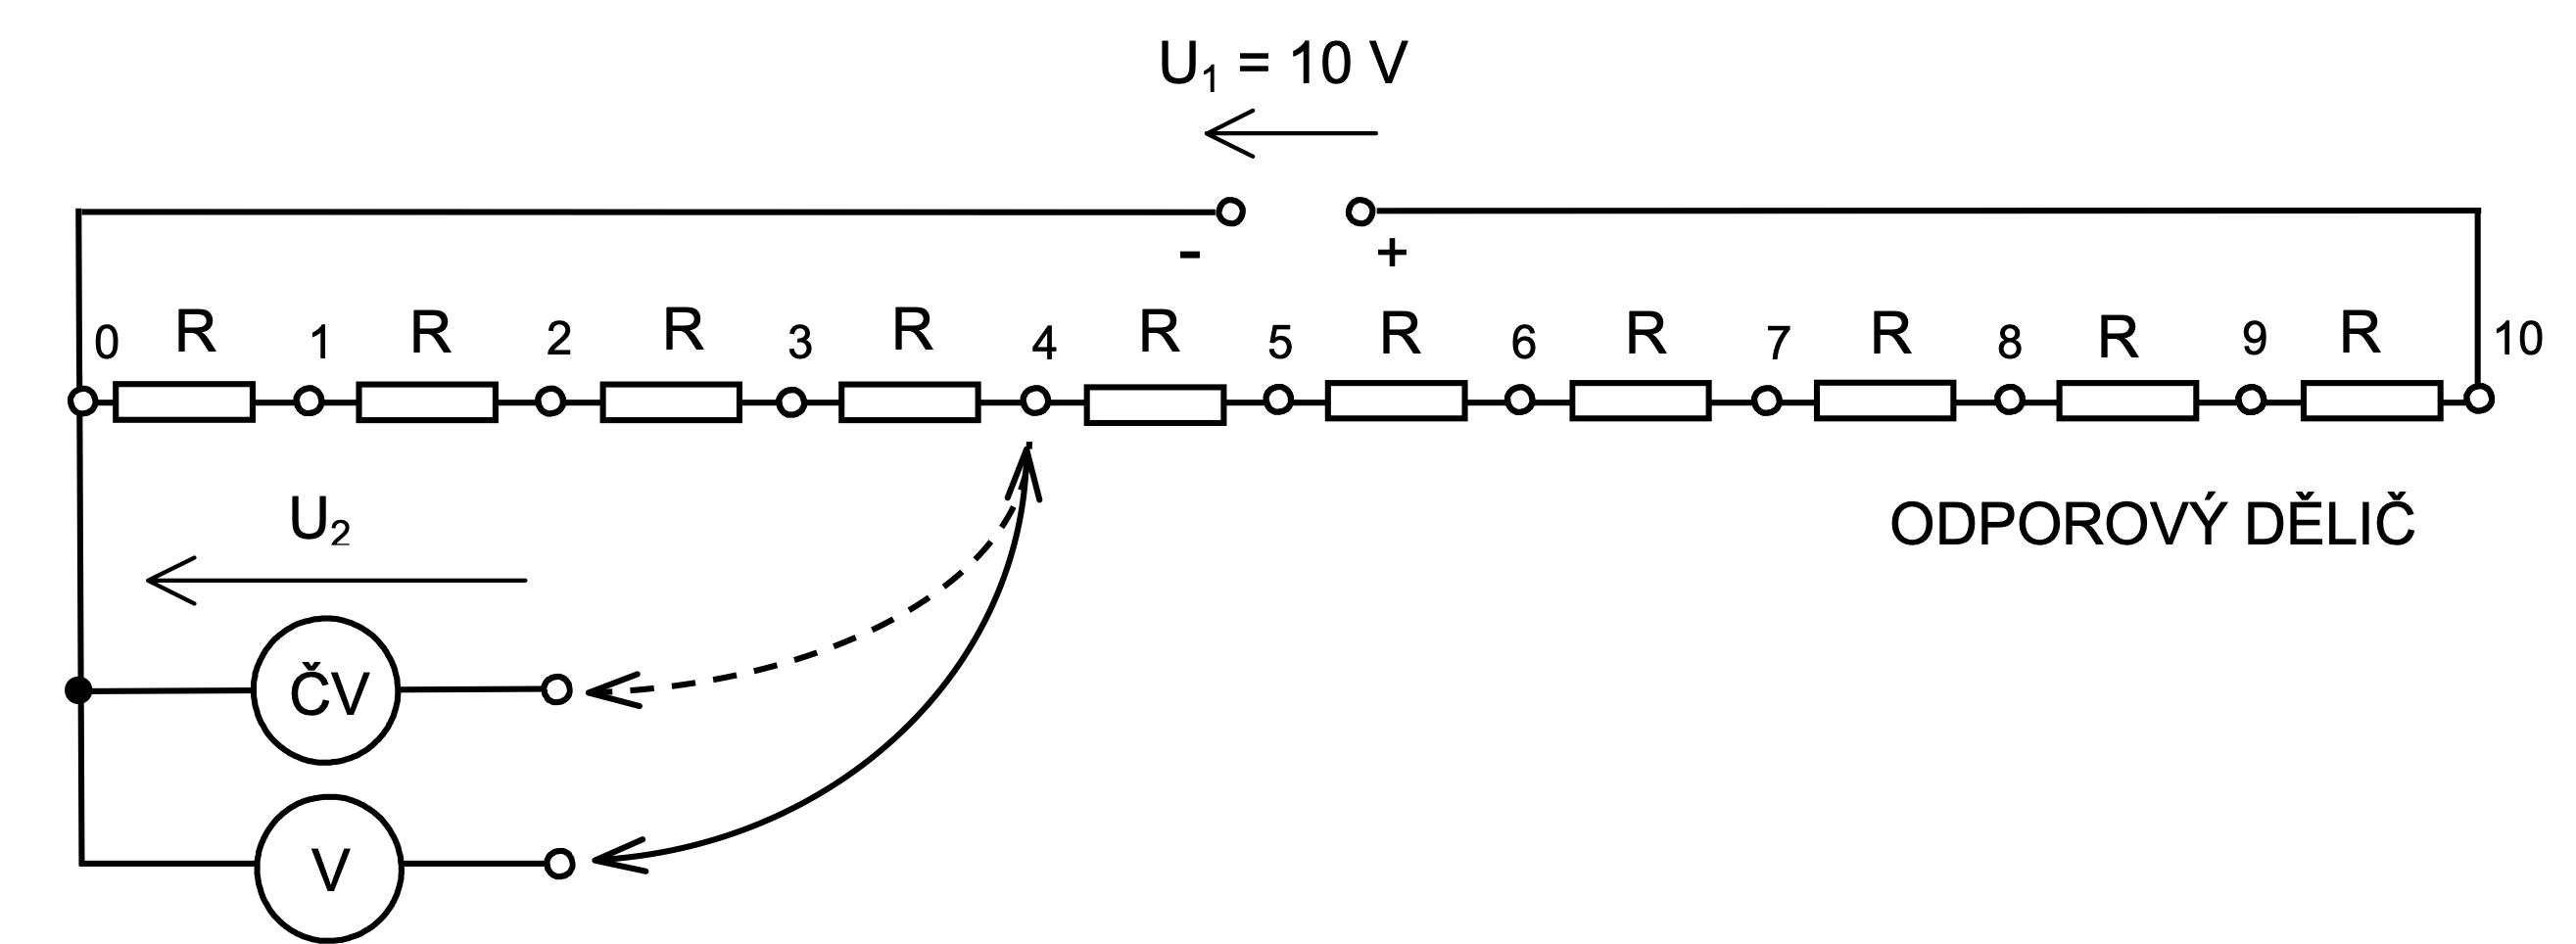
\includegraphics[width=.8\textwidth]{schema.png}
    \caption{Zapojení obvodu \cite{navod}}
    \label{fig:zapojeni}
\end{figure}


\section{Seznam použitých přístrojů}
\begin{itemize}
    \item Dělič napětí s devíti odbočkami
    \item Stolní multimetr HP 34401 A, přesnost $\pm$\,0,0035\,\% z údaje a $\pm$\,0,005\,\% rozsahu
    \item Ručičkový voltmetr, třída přesnosti 0,5\,\%, rozsah 12\,V
\end{itemize}

\section{Teoretický úvod}
Při měření napětí na odporovém děliči dochází k chybě měření způsobené vnitřním odporem měřiče. Odporový dělič si lze nahradit náhradním zapojením zdroje napětí a sériového rezistoru. Napětí ideálního zdroje napětí je rovno napětí na děliči naprázdno a vnitřní odpor odpovídá paralelní kombinaci rezistorů v děliči napětí. Po připojení multimetru k tomuto náhradnímu zapojení vznikne další dělič napětí a to mezi vnitřním rezistorem náhradního zapojení a vnitřním odporem měřidla. Při použití kvalitnějších měřidel se se vnitřní odpor blíží vůči odporům rezistorů v děliči k nekonečnu. Nicméně při použití starších, levnějších nebo ručičkových měřidel dochází k chybě měření, která právě závisí na jeho vnitřním odporu. 


\section{Naměřené hodnoty}
Dle odečtu z videa byly naměřeny hodnoty zobrazené v tabulce \ref{tab:hodnoty} a zobrazené v grafu \ref{graf:hodnoty}.

\begin{table}[h!]
    \centering
    \begin{tabular}{|c|c|c|c|}
    \hline
        \rule{0pt}{2.5ex} Odbočka & HP 34401 A $\frac{U}{V}$ & Ručičkový voltmetr $\frac{U}{V}$&Dělící poměr\\[.7ex] \hline\hline
        10 &	9,9919 &	9,9 &   1   \\\hline
        9 &	8,9827 &	7,2 &   0,9 \\\hline
        8 &	7,9659 &	5,6 &   0,8 \\\hline
        7 &	6,9716 &	4,5 &   0,7 \\\hline
        6 &	5,9761 &	3,7 &   0,6 \\\hline
        5 &	4,9781 &	3,05&   0,5 \\\hline
        4 &	3,9753 &	2,5 &   0,4 \\\hline
        3 &	2,9823 &	1,95&   0,3 \\\hline
        2 &	1,9867 &	1,6 &   0,2 \\\hline
        1 &	0,9925 &	0,8 &   0,1 \\\hline
    \end{tabular}
    \caption{Naměřené hodnoty}
    \label{tab:hodnoty}
\end{table}

\begin{graf}
    \centering
    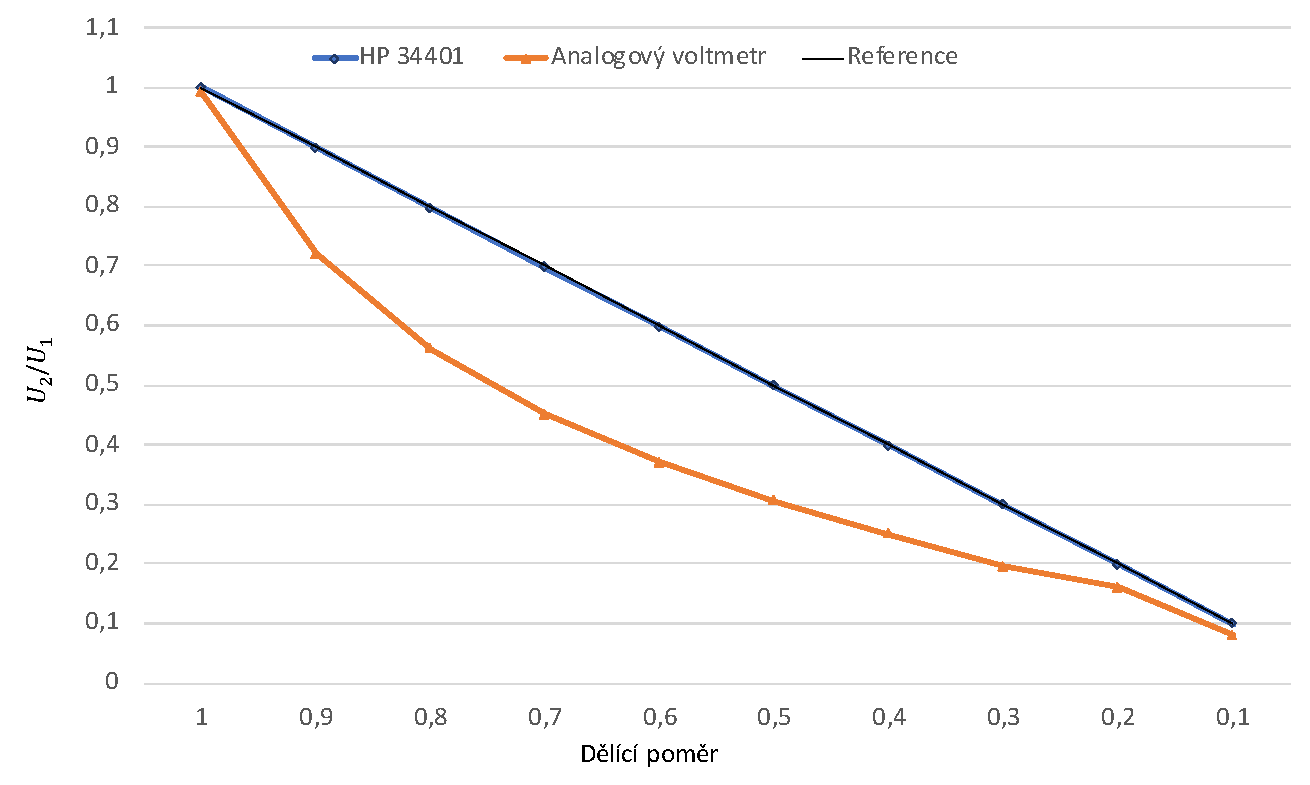
\includegraphics[width = .8\textwidth]{graf1.pdf}
    \caption{Vynesené hodnoty číslicového a ručičkového voltmetru doplněné o referenční úsečku ideálních hodnot}
    \label{graf:hodnoty}
\end{graf}


\section{Zpracování naměřených hodnot}

\subsection{Výpočet výstupního odporu děliče}
Výstupní odpor děliče bude počítán pro dělící poměr 0,5. Dělící poměr d~=~0,5 - odpovídající číslu odbočky 5 - byl vybrán kvůli největšímu rozdílu mezi napětím číslicového voltmetru \ucv ~a~napětím ručičkového \urv.

\begin{table}[h!]
    \begin{tabular}{lll}
        \ucv    & 4,9781\,V &  - měřené napětí je bráno jako napětí naprázdno \\
        \urv    & 3,05\,V    &  - napětí měřené ručičkovým voltmetrem\\
        \rrv    & 5\,000\,$\Omega$V$^{-1}$ $\cdot$ 12\,V = 60\,$\textrm{k}\Omega$ & - vnitřní odpor ručičkového voltmetru\\
    \end{tabular}
\end{table}

Tímto jsme získali hodnotu napětí naprázdno a napětí, pokud na výstup děliče připojíme rezistor s odporem 60\,$\textrm{k}\Omega$. Popis použitých proměnných je v tabulce \ref{tab:prom}.
\begin{table}[h!]
    \centering
    \begin{tabular}{l|l}
        \ucv ~= \un & napětí děliče naprázdno resp. napětí měřené číslicovým voltmetrem \\
        \urv & napětí měřené ručičkovým voltmetrem \\
        \rrv & vnitřní odpor ručičkového voltmetru \\
        \rd  & odpor napěťového děliče R$_1$\,||\,R$_2$\\
    \end{tabular}
    \caption{Význam proměnných}
    \label{tab:prom}
\end{table}

Díky použití náhradního zapojení můžeme obvod zjednodušit na ideální zdroj napětí o velikosti U$_{0}$, která odpovídá velikosti \ucv ~a sériově k němu zapojený rezistor o velikosti \rd ~resp. $R_1$\,||\,$R_2$. Po připojení ručičkového voltmetru se z \rd ~a \rrv ~vytvoří napěťový dělič a \urv ~je hodnota napětí na děliči vůči zemi. \urv ~odpovídá rovnici
\begin{equation}
    \eurv = \eucv \frac{\errv}{\eurv+\erd}.
\end{equation}

Poté si jen stačí vyjádřit \rd:
\begin{equation*}
    \begin{split}
        \eucv\cdot\errv &= \eurv\cdot\errv+\eurv\cdot\erd\\
        \erd &= \frac{(\eucv-\errv)\errv}{\eurv} \\
    \end{split}
\end{equation*}
\begin{equation}
    \erd = \errv\left(\frac{\eucv}{\eurv}-1\right).
    \label{eq:rd}
\end{equation}

Pro tuto hodnotu nám výstupní odpor napěťového děliče po dosazení vyjde \rd ~= 37\,929,8\,$\Omega$. Při použití vzorce z rovnice \ref{eq:rd} pro ostatní dělící poměry resp. odbočky v děliči napětí dostaneme následující hodnoty:
\begin{table}[h!]
    \centering
    \begin{tabular}{|c|r|}
        \hline
        \rule{0pt}{2.5ex} Dělící poměr & \rd ~$\frac{R}{\Omega}$\\[.7ex] \hline\hline
        1,0   & 557,0     \\\hline
        0,9 & 14\,855,8   \\\hline
        0,8 & 25\,348,9   \\\hline
        0,7 & 32\,954,7   \\\hline
        0,6 & 36\,909,7   \\\hline
        0,5 & 37\,929,8   \\\hline
        0,4 & 35\,407,2   \\\hline
        0,3 & 31\,763,1   \\\hline
        0,2 & 14\,501,3   \\\hline
        0,1 & 14\,437,5   \\\hline
    \end{tabular}
    \caption{Výstupní odpor děliče napětí v závislosti na dělícím poměru}
    \label{tab:odpory}
\end{table}

Data z tabulky \ref{tab:odpory} jsou vynesena v grafu \ref{graf:odpory} níže.
\begin{graf}
\centering
    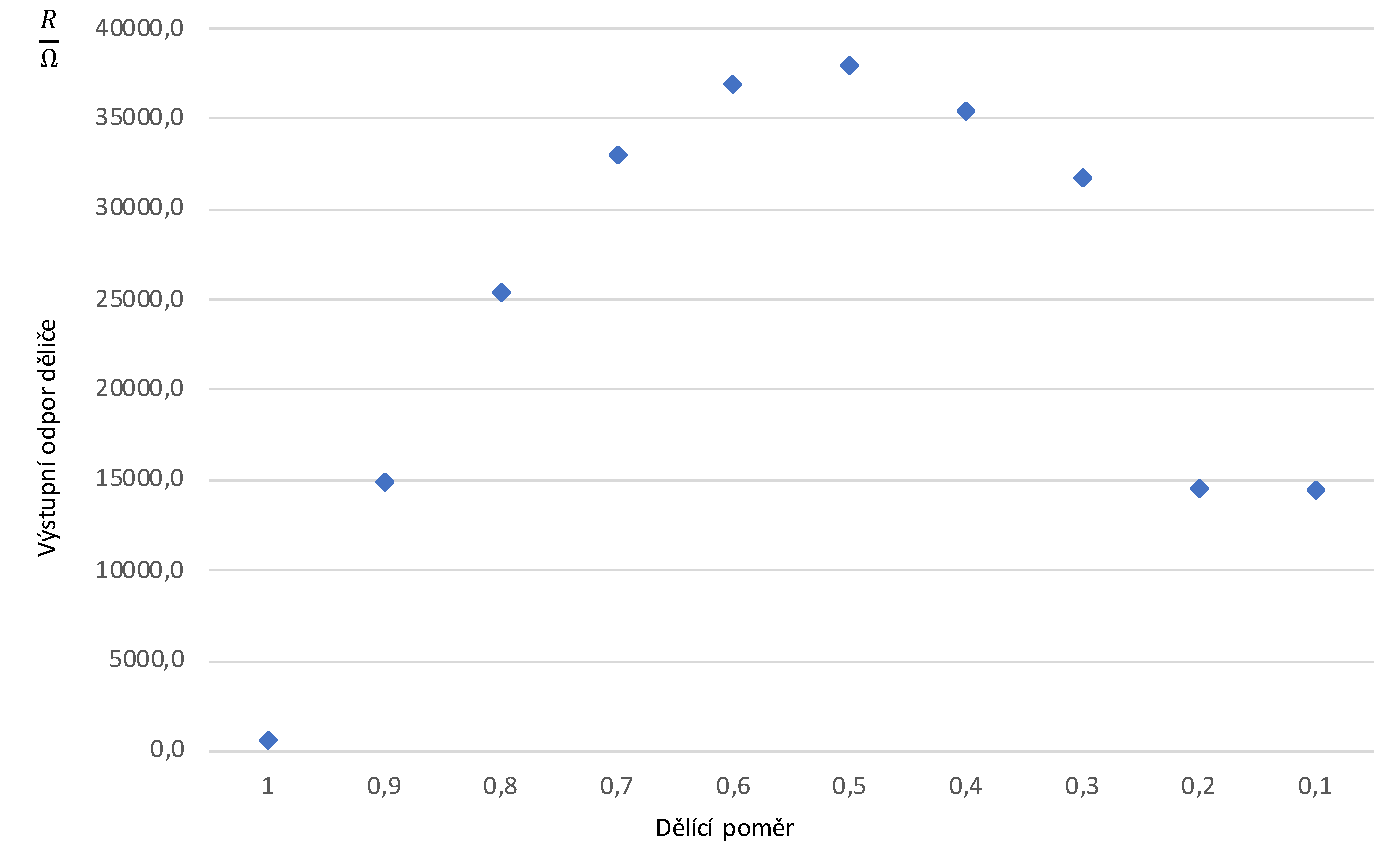
\includegraphics[width = 0.8\textwidth]{graf3.pdf}
    \caption{Výstupní odpor děliče napětí v závislosti na dělícím poměru}
    \label{graf:odpory}
\end{graf}


\subsection{Výpočet rozšířené nejistoty typu B}
Ručičkový voltmetr, rozsah 12\,V, TP\,=\,0,5\,\%:
\begin{equation*}
    u(\eurv)=\frac{TP\cdot rozsah}{100\sqrt{3}}=\frac{0,5\cdot12}{100\sqrt{3}}=0,035\,\textrm{V}.
\end{equation*}

Nejistota vnitřního odporu \rrv ~ručičkového voltmetru s tolerancí 0,2\,\%:
\begin{equation*}
    u(\errv) = \frac{TP\cdot rozsah}{100\cdot\sqrt{3}} = \frac{0,2\cdot 60\cdot 10^3}{100\cdot \sqrt{3}} = 69,3\,\Omega.
\end{equation*}

Číslicový voltmetr, chyba $\delta_1\,=\,\pm$\,0,0035\,\% z údaje \ucv \,=\,49781 a $\delta_2\,=\,\pm$\,0,005\,\% rozsahu $M_{CV}$\,=\,10\,V:
\begin{equation*}
    u(\eucv)=\frac{\delta_1\cdot\eucv + \delta_2\cdot M_{CV}}{100\sqrt{3}}=\frac{0,0035\cdot 4,9781 + 0,0005\cdot 10}{100\sqrt{3}}=1,29\cdot 10^{-4}\,\textrm{V}.
\end{equation*}

Rozšířená nejistota typu B, $k_r$\,=\,2:
\begin{equation*}
    \begin{split}
        u(\erd)&=\sqrt{\left( \frac{\partial \erd}{\partial\eucv}u(\eucv) \right)^2+\left( \frac{\partial \erd}{\partial\eurv}u(\eurv) \right)^2+\left( \frac{\partial \erd}{\partial\errv}u(\errv) \right)^2}\\
        u(\erd)&=\sqrt{\left( \frac{\errv}{\eucv}u(\eucv) \right)^2+\left( \frac{\errv\eucv}{\eurv}u(\eurv) \right)^2+\left( \frac{\eucv-\eurv}{\eurv}(\errv) \right)^2}\\
        u(\erd)&=\sqrt{\left( \frac{60\cdot10^{3}}{3,05}\cdot(1,29\cdot 10^{-4}) \right)^2+\left( \frac{60\cdot 10^3\cdot 4,9781}{3,05^2}\cdot(0,035) \right)^2+\left( \frac{4,9781-3,05}{3,05}\cdot(69,3) \right)^2}\,\Omega\\
        u(\erd)&=1124,6\,\Omega\\
        u(\erd)&=k_r\cdot u(\erd)=2\cdot 1124,6\,\Omega = 2249,28\,\Omega.\\
    \end{split}
\end{equation*}


\section{Závěrečné vyhodnocení}
Měřením bylo potvrzeno, že některé voltmetry nelze považovat za ideální. Jejich přítomnost v obvodu může způsobit chybu měření napětí a v případě dalších měřidel chybu měření dalších veličin. Hodnoty měřené číslicovým voltmetrem byly velice blízké skutečné hodnotě naprázdno a~proto jsme mohli vnitřní odpor voltmetru považovat za nekonečný a odporový dělič za nezatížený.

Výstupní odpor napěťového děliče nám vyšel \rd \,=\,37\,929,8\,$\pm$\,2249\,$\Omega$.





%--- LITERATURA a~ZDROJE (povinne) ---
\clearpage
\renewcommand{\refname}{Seznam použité literatury a~zdrojů informací} 
%\section*{Seznam použité literatury a~zdrojů informací}
\phantomsection %pridej odkaz do PDF zalozek
\addcontentsline{toc}{section}{Seznam použité literatury a~zdrojů informací}

\begin{thebibliography}{99}

%----------------------------------------------------
\subsection*{Seznam použitých internetových zdrojů}
    \bibitem{navod} Návod k laboratorní úloze
    
\end{thebibliography}




\end{document}